\section{Methodology}
\label{sec:method}

% Model numbers below come from the run records through
% scripts/report/a2_method_tables.py; regenerate instead of editing them.
% Generated by scripts/report/a2_method_tables.py from the U-Net training summary, the ablation results and the model code. Do not edit.
\newcommand{\unetParameters}{7{,}763{,}272}
\newcommand{\unetDepth}{4}
\newcommand{\unetWidthFirst}{32}
\newcommand{\unetWidthLast}{512}
\newcommand{\unetDownsample}{16}
\newcommand{\unetBottleneckHeight}{15}
\newcommand{\unetBottleneckWidth}{20}
\newcommand{\unetWorkers}{4}
\newcommand{\deeplabParameters}{39{,}635{,}528}
\newcommand{\deeplabLibraryParameters}{42{,}004{,}074}
\newcommand{\deeplabLibraryCategories}{21}
\newcommand{\deeplabLibraryMiou}{66.4}
\newcommand{\deeplabHeadRate}{$10^{-3}$}
\newcommand{\deeplabBackboneRate}{$10^{-4}$}
\newcommand{\deeplabBatch}{4}
\newcommand{\parameterRatio}{5.1}
\newcommand{\unetLearningRate}{$10^{-3}$}
\newcommand{\unetWeightDecay}{$10^{-4}$}
\newcommand{\unetEpochs}{40}
\newcommand{\unetWarmupEpochs}{5}
\newcommand{\unetSeed}{42}
\newcommand{\unetDevice}{RTX 4060 Laptop GPU}
\newcommand{\unetTorchVersion}{2.14.0}
\newcommand{\unetCudaVersion}{13.0}
\newcommand{\deeplabAtrousRates}{12, 24 and 36}
\newcommand{\deeplabAsppChannels}{256}
\newcommand{\deeplabBackboneChannels}{2{,}048}
\newcommand{\deeplabOutputStride}{8}
\newcommand{\deeplabFeatureHeight}{30}
\newcommand{\deeplabFeatureWidth}{40}
\newcommand{\deeplabDevice}{RTX 4060 Ti}
\newcommand{\deeplabTorchVersion}{2.14.0}
\newcommand{\deeplabCudaVersion}{12.6}


\subsection{Training and evaluation pipeline}
\label{sec:pipeline}
\figref{fig:pipeline} shows the pipeline that both models share. The raw
SUIM pairs pass the audit of \secref{sec:eda}, and the remaining pairs are
preprocessed as described in \secref{sec:preprocessing} and served in
batches by the data loader. The model maps each image to eight logits per pixel,
and the loss compares them with the class-index mask. AdamW updates the weights
after each group of accumulated batches, with a learning rate that rises
linearly during a warm-up and then follows a cosine decay. After every epoch the
model predicts the validation set, and the checkpoint with the highest
validation mIoU is kept. A prediction assigns each pixel the class with the
highest logit. The only post-processing step resizes the logits to the mask grid
with bilinear interpolation before this argmax when the two sizes differ; in our
runs the model output and the mask both have
$\suimInputHeight\times\suimInputWidth$ pixels, so the step changes nothing. We
use no conditional random field, test-time augmentation or other refinement.
Evaluation accumulates a confusion matrix over all pixels of a split and derives
the metrics of \secref{sec:metrics} from it.

\begin{figure}[htbp]
\centering
\begin{tikzpicture}[
  stage/.style={draw, rounded corners=2pt, align=center, font=\scriptsize,
    text width=2.2cm, minimum height=1.3cm, inner sep=2pt},
  flow/.style={-{Stealth[length=4pt]}, thick},
  node distance=0.32cm]
\node[stage] (raw) {\textbf{Raw data}\\JPEG images,\\RGB BMP masks};
\node[stage, right=of raw] (prep) {\textbf{Preprocessing}\\audit, decode,\\resize,\\normalize, flip};
\node[stage, right=of prep] (load) {\textbf{Data loader}\\split files,\\shuffled batches};
\node[stage, right=of load] (model) {\textbf{Model}\\U-Net or\\DeepLabV3};
\node[stage, right=of model] (loss) {\textbf{Loss}\\CE or\\CE + Dice};
\node[stage, right=of loss] (opt) {\textbf{Optimization}\\AdamW, warm-up\\and cosine,\\accumulation};
\node[stage, below=0.75cm of model] (pred) {\textbf{Prediction}\\argmax over\\eight classes};
\node[stage, right=of pred] (post) {\textbf{Post-processing}\\logit resize\\if sizes differ};
\node[stage, right=of post] (eval) {\textbf{Evaluation}\\pooled confusion\\matrix, mIoU,\\mDice};
\draw[flow] (raw) -- (prep);
\draw[flow] (prep) -- (load);
\draw[flow] (load) -- (model);
\draw[flow] (model) -- (loss);
\draw[flow] (loss) -- (opt);
\draw[flow] (opt.north) to[bend right=14] node[above, font=\scriptsize] {weight update} (model.north);
\draw[flow] (model) -- (pred);
\draw[flow] (pred) -- (post);
\draw[flow] (post) -- (eval);
\end{tikzpicture}
\caption{Training and evaluation pipeline for SUIM segmentation. The top row is
the training path; the bottom row turns logits into predictions and scores
them, on the validation set after every epoch and on the test set once.}
\label{fig:pipeline}
\end{figure}

The data loader never holds the dataset in memory. Images are read, decoded and
resized from disk only when a batch is requested, by \unetWorkers{} worker
processes that prepare the next batches while the GPU trains on the current
one, and pinned host memory speeds up the copy to the device. Shuffling uses a
generator seeded from the run seed and the epoch number, so the batch order can
be reproduced and a resumed run continues with the same order. The physical
batch stays small to limit memory use, and gradients are accumulated over
several batches before each optimizer step (\secref{sec:training}). The
same code also runs on several GPUs: the training set is then sharded across
devices, gradients are synchronized only at optimizer steps, and validation
still runs on the full set on one device.

We wrote the data audit, the duplicate search, the dataset class and its
transforms, the U-Net, the combined cross-entropy and Dice loss, the metrics,
and the training loop with gradient accumulation, the learning-rate schedule,
checkpointing and resume. Libraries provide the rest: PyTorch supplies the
layers, automatic differentiation, the AdamW optimizer, the cross-entropy loss,
data loading and distributed training; torchvision supplies the DeepLabV3
architecture and its pretrained weights; Pillow decodes and resizes images;
NumPy decodes the masks; and scikit-learn provides the stratified group split.

\subsection{Model architectures}
\label{sec:models}

\subsubsection{U-Net baseline}
The baseline is a U-Net \cite{unet} that we implemented ourselves and train from
random initialization. Each encoder level applies two $3\times3$ convolutions,
each followed by batch normalization and a ReLU, and then halves the resolution
with $2\times2$ max pooling. This repeats \unetDepth{} times, and one more block
of two convolutions forms the bottleneck. The number of channels starts at
\unetWidthFirst{} and doubles at every level up to \unetWidthLast{} at the
bottleneck, where a $\suimInputHeight\times\suimInputWidth$ input has shrunk to
$\unetBottleneckHeight\times\unetBottleneckWidth$. The decoder mirrors the
encoder: a $2\times2$ transposed convolution with stride 2 doubles the
resolution and halves the channels, a skip connection concatenates the result
with the encoder features of the same resolution, and another block of two
convolutions fuses them. A final $1\times1$ convolution maps the
\unetWidthFirst{} channels to eight logits per pixel at the input resolution.
All convolutions are padded, so the output has the size of the input, and both
input sides must be divisible by \unetDownsample{}, which holds for our input
size. Compared with the original U-Net, our version uses padded instead of
unpadded convolutions, adds batch normalization, and starts with half as many
channels. It has \unetParameters{} parameters. \figref{fig:unet} shows
the resulting network.

\begin{figure}[htbp]
\centering
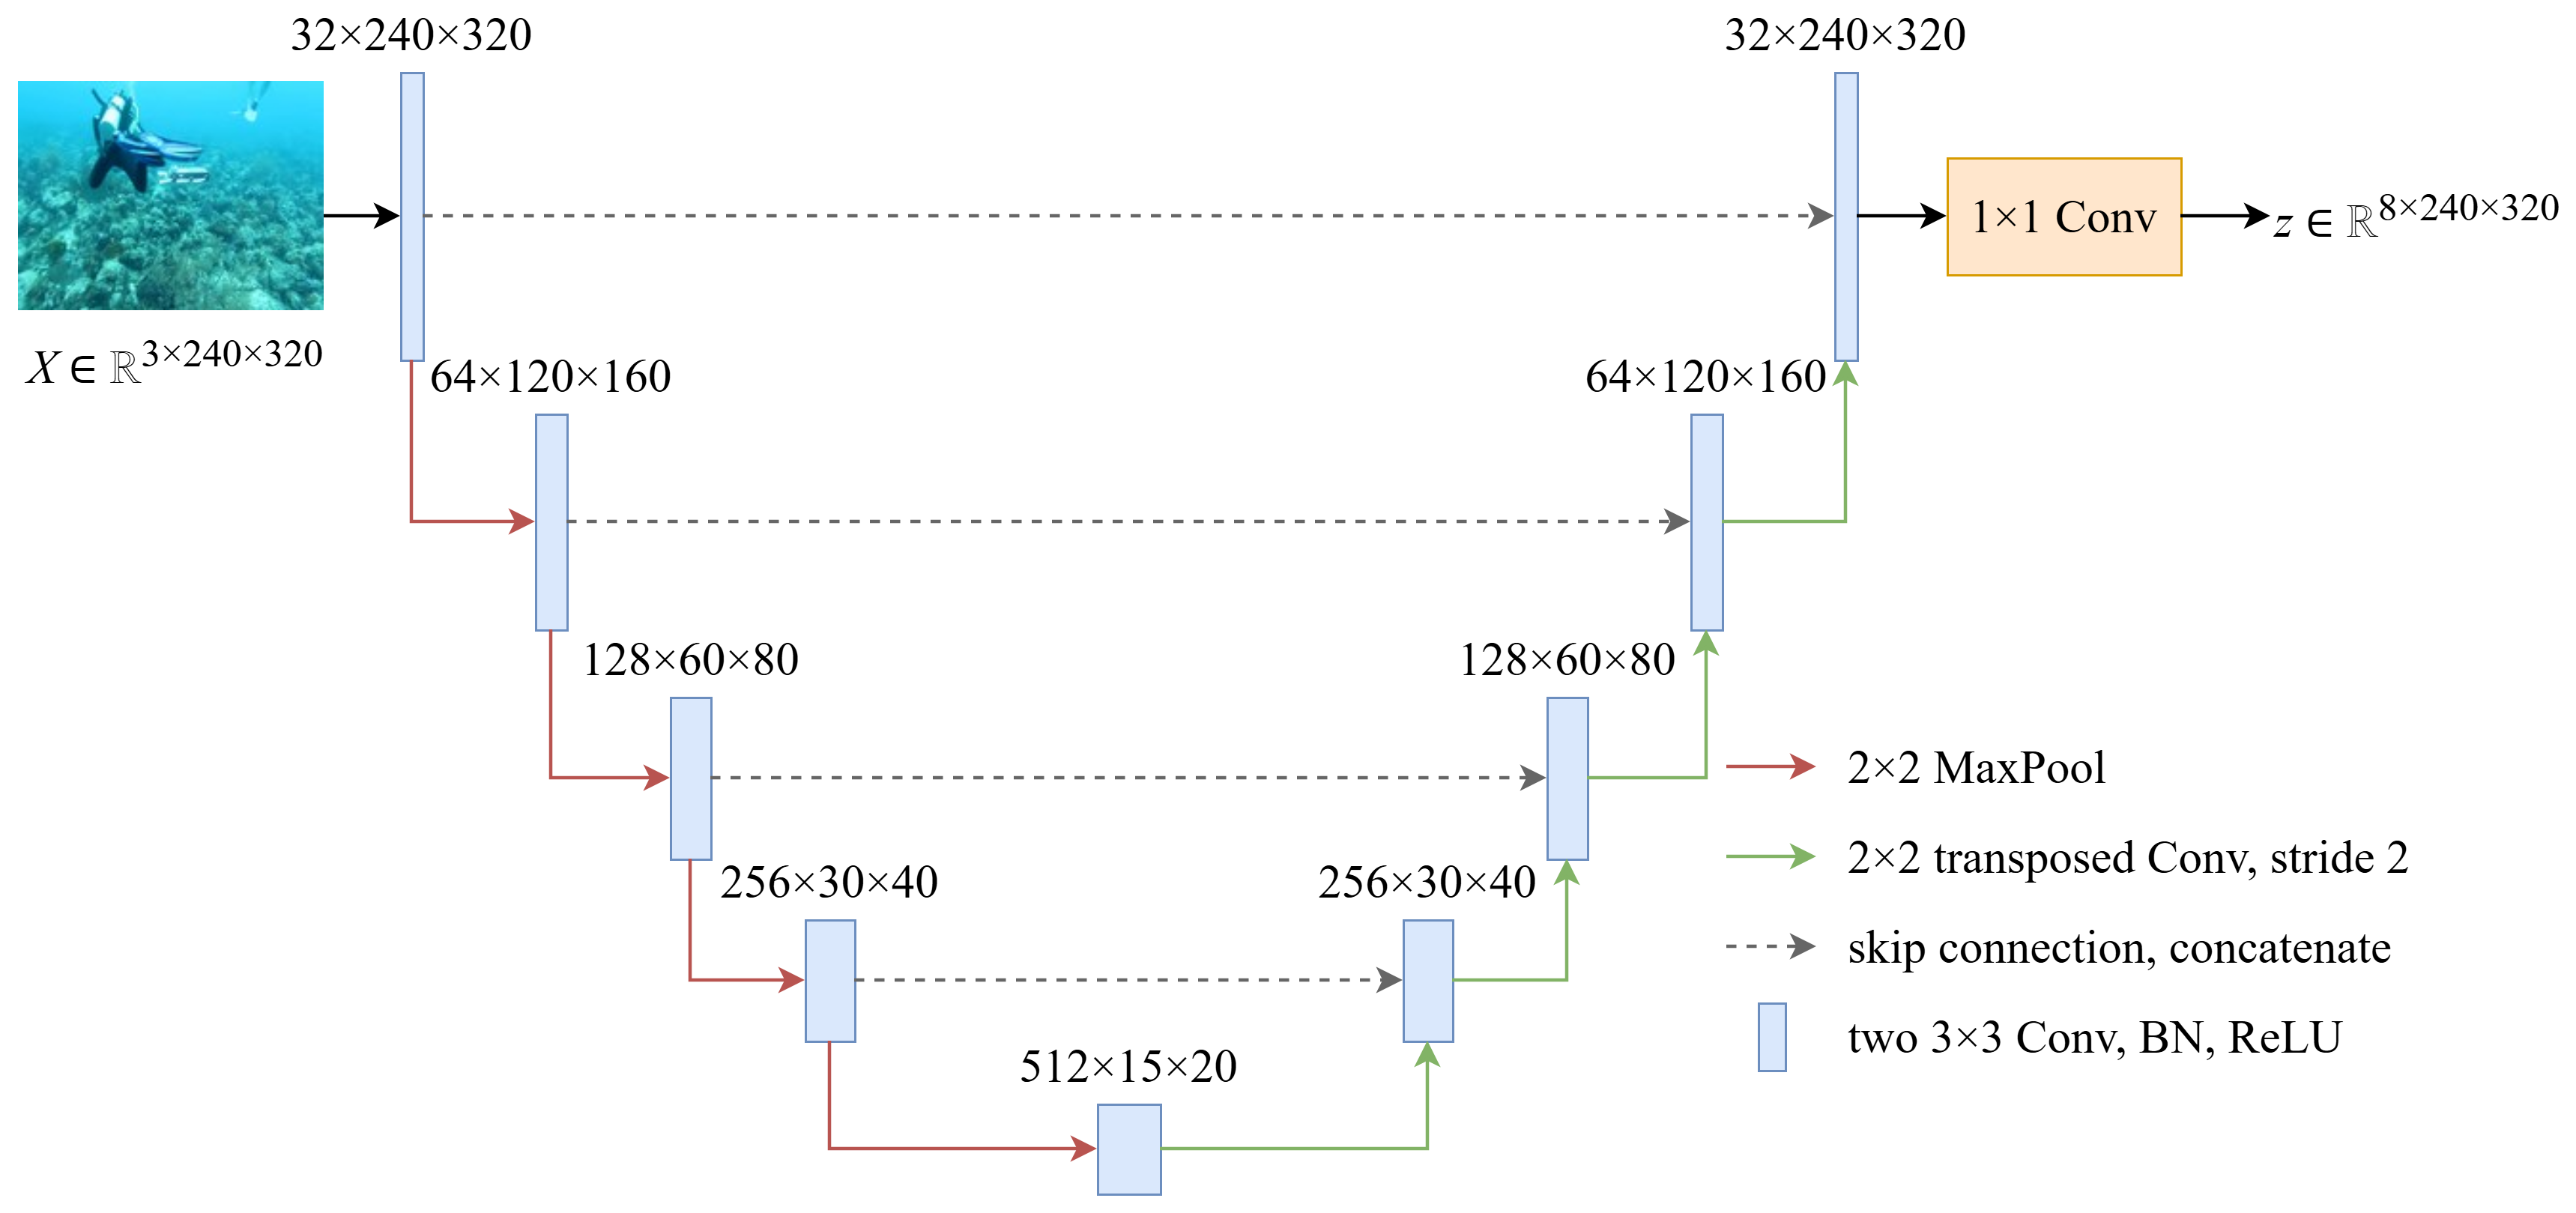
\includegraphics[width=0.95\linewidth]{Images/models/unet.png}
\caption{The U-Net baseline. Each bar is a block of two $3\times3$
convolutions, each followed by batch normalization and ReLU, labelled with its
output channels and resolution for our input size. Every layer is written by
the group and starts from random weights.}
\label{fig:unet}
\end{figure}

The skip connections carry full-resolution features to the output, which helps
the model place boundaries and keep small objects such as fish and divers. Its
main limitation for this task is that it starts without any knowledge of
natural images and must learn all its features from \suimTrainImages{} training
images. Its context is also limited, because each bottleneck feature sees only
a part of the image, so it has fewer global cues than DeepLabV3 for telling reef
from rock and sea floor.

\subsubsection{Pretrained DeepLabV3}
The pretrained model is DeepLabV3 \cite{deeplabv3} with a ResNet-50 backbone,
taken together with its weights from torchvision \cite{torchvision}. In the
last two stages of the backbone, atrous (dilated) convolutions replace the
striding, so the output stride is \deeplabOutputStride{} instead of 32: a
$\suimInputHeight\times\suimInputWidth$ input yields a
$\deeplabFeatureHeight\times\deeplabFeatureWidth$ feature map with
\deeplabBackboneChannels{} channels. Atrous convolution enlarges the receptive
field without reducing the resolution further. On top of the backbone, the
atrous spatial pyramid pooling (ASPP) module runs five branches in parallel: a
$1\times1$ convolution, three $3\times3$ atrous convolutions with rates
\deeplabAtrousRates{}, and a global average pooling branch that adds
image-level context. Each branch has \deeplabAsppChannels{} channels. Their
outputs are concatenated, projected back to \deeplabAsppChannels{} channels by a
$1\times1$ convolution with dropout, and refined by a $3\times3$ convolution. A
final $1\times1$ convolution produces the class logits, which are upsampled
bilinearly by a factor of \deeplabOutputStride{} to the input size. On a map of
only \deeplabFeatureHeight{} rows, most outer taps of the large-rate filters fall
on zero padding, so these branches act partly as $1\times1$ convolutions; the
DeepLabV3 paper describes this effect and relies on the image pooling branch for
global context in such cases \cite{deeplabv3}. \figref{fig:deeplab} shows
the network with the changes described below.

\begin{figure}[htbp]
\centering
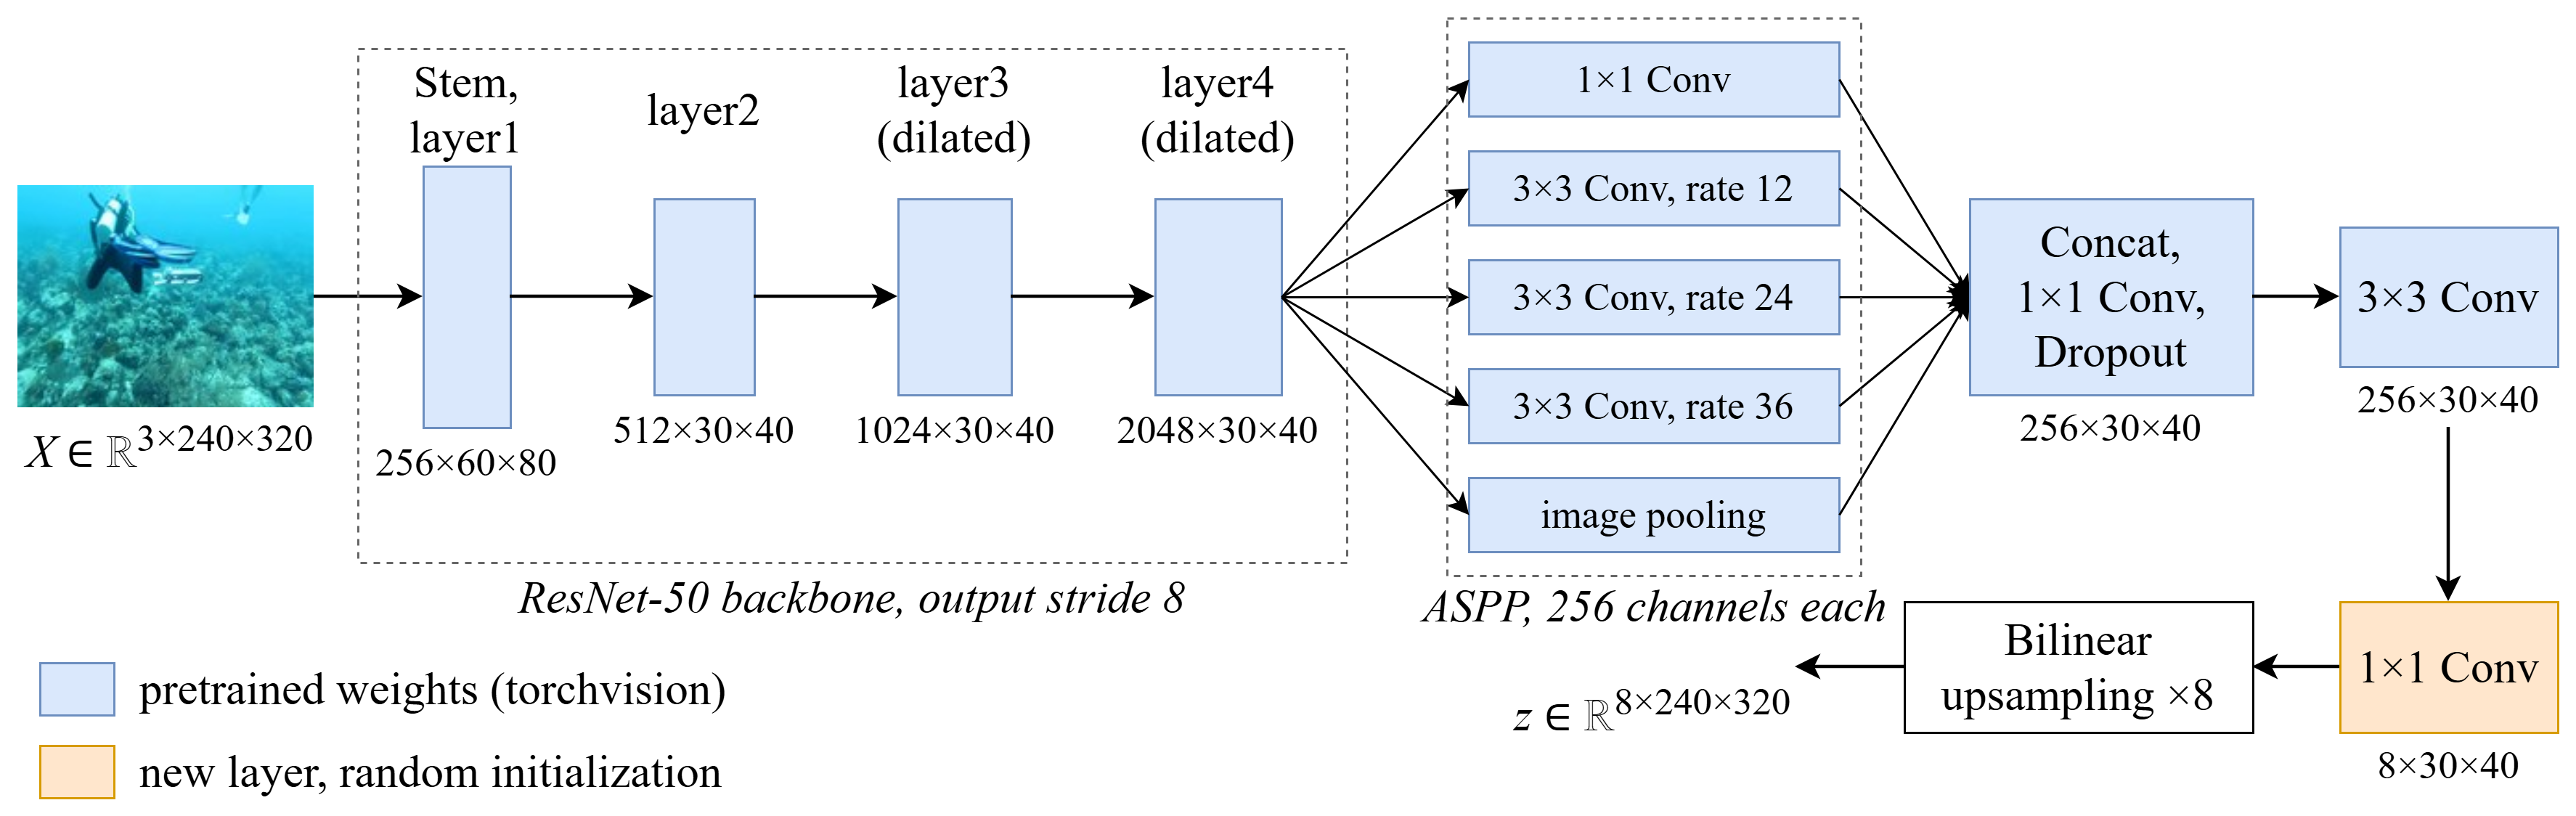
\includegraphics[width=\linewidth]{Images/models/deeplabv3.png}
\caption{DeepLabV3 as used in this work. Blue layers start from the
torchvision weights pretrained on COCO with the Pascal VOC categories; the
orange output layer replaces the original one. The white box has no weights.
Batch normalization statistics are fixed in all layers, and the auxiliary head
of the torchvision model is removed.}
\label{fig:deeplab}
\end{figure}

The weights, named \codepath{COCO_WITH_VOC_LABELS_V1} in torchvision, were
trained on a subset of COCO that keeps only the Pascal VOC categories, giving
\deeplabLibraryCategories{} output classes including background. Torchvision
reports \deeplabLibraryMiou\% mIoU for them on COCO val2017 with VOC labels. We
replace the last $1\times1$ convolution, which predicts
\deeplabLibraryCategories{} classes, with a new randomly initialized one with
eight outputs, and we remove the auxiliary head that torchvision attaches to the
third backbone stage, because we use no auxiliary loss. All other weights,
including the ASPP module, start from the pretrained values. The model keeps
\deeplabParameters{} parameters, against \deeplabLibraryParameters{} in the
torchvision version with both heads, and all of them are trained. The
architecture and weights come from torchvision; we wrote the wrapper that
replaces the head, removes the auxiliary branch, fixes the batch normalization
statistics, and splits the parameters into two learning-rate groups
(\secref{sec:finetune}).

Pretraining gives the backbone general features for edges, textures and object
parts, and ASPP adds context at several scales, which should help on large
classes such as reef and sea floor. The limits of the model mirror the
strengths of U-Net. Logits are computed at one eighth of the input resolution
and upsampled without skip connections, so thin structures and boundaries are
blurred, which matters for small classes such as fish and plants. The
pretraining images were taken above water, so colour cast and turbidity are new
to the model. DeepLabV3 also has \parameterRatio{} times as many parameters as
our U-Net (\tabref{tab:model-summary}).

% Generated by scripts/report/a2_method_tables.py from the U-Net training summary, the ablation results and the model code. Do not edit.
\begin{table}[htbp]
\centering\small
\caption{Compared models. Implementation states whether the group wrote the
model or used a library.}
\label{tab:model-summary}
\begin{tabular}{llllr}
\toprule
Model & Role & Initialization & Implementation & Parameters\\
\midrule
U-Net & Baseline & Random & Group & 7{,}763{,}272\\
DeepLabV3 (ResNet-50) & Pretrained & COCO, VOC labels & torchvision, new head & 39{,}635{,}528\\
\bottomrule
\end{tabular}
\end{table}


\subsection{Fine-tuning procedure}
\label{sec:finetune}
We fine-tune the whole network rather than only the head. Its parameters form
two groups with different learning rates. The backbone uses
\deeplabBackboneRate{}, and the head, made of the ASPP module, the $3\times3$
convolution and the new output layer, uses \deeplabHeadRate{}. The backbone
already provides useful features, so a small rate adapts it to underwater
images without destroying what it learned, while the new output layer starts
from random weights and needs a larger rate. The pretrained ASPP layers belong
to the head group as well, since they must adapt to a new set of classes. Both
groups follow the same warm-up and cosine schedule (\secref{sec:training}),
which scales their rates by the same factor at every step. The two rates were
fixed in the Dataset Proposal and were not tuned.

Batch normalization does not follow standard training. In every normalization
layer of the backbone and the head, the running mean and variance stay at their
pretrained values during training and evaluation, while the scale and shift
parameters are still learned. With a physical batch of \deeplabBatch{} images,
batch statistics would be noisy, and gradient accumulation does not help
because it does not enlarge the batch that a normalization layer sees. Fixing
the statistics also keeps the features consistent with the normalization used
in pretraining, which is why the inputs are normalized with the ImageNet
constants (\secref{sec:preprocessing}).

\subsection{Loss and evaluation metrics}
\label{sec:metrics}
Both models are trained with pixel-wise cross-entropy, averaged over all $N$
pixels of a batch without class weights,
\begin{equation}
\mathcal{L}_{\mathrm{CE}}=-\frac{1}{N}\sum_{i=1}^{N}\log p_{i,y_i},
\end{equation}
where $p_{i,k}$ is the softmax probability of class $k$ at pixel $i$ and $y_i$
is its true class. The controlled experiment adds a soft Dice term. For image
$n$ of a batch of $B$ images and class $k$ of the $K=8$ classes, with $g_{i,k}$
equal to one if pixel $i$ belongs to class $k$ and zero otherwise,
\begin{equation}
D_{n,k}=\frac{2\sum_{i}p_{i,k}\,g_{i,k}+\epsilon}{\sum_{i}p_{i,k}+\sum_{i}g_{i,k}+\epsilon},
\qquad
\mathcal{L}_{\mathrm{Dice}}=1-\frac{1}{BK}\sum_{n=1}^{B}\sum_{k=1}^{K}D_{n,k},
\end{equation}
where the sums run over the pixels of image $n$ and $\epsilon$ is a small
constant that prevents division by zero. The combined loss is
$\mathcal{L}=0.5\,\mathcal{L}_{\mathrm{CE}}+0.5\,\mathcal{L}_{\mathrm{Dice}}$.
Every class has the same weight in the Dice term regardless of how many pixels
it covers, which is why we expect it to help the rare classes. The term is
computed per image and then averaged, so its value does not depend on how
batches are grouped for gradient accumulation. Classes absent from an image are
kept in the average. For such a class the numerator is only $\epsilon$, so its
Dice score is close to zero unless the predicted probabilities sum to less than
$\epsilon$. These classes therefore add an almost constant amount to the loss
with little gradient, and the Dice term acts mainly through the classes present
in each image.

Evaluation uses a $K\times K$ confusion matrix $C$ whose entry $C_{jk}$ counts
the pixels of true class $j$ predicted as class $k$. The counts are accumulated
over every pixel of every image in a split before any score is computed. For
class $k$, $\mathrm{TP}_k=C_{kk}$, $\mathrm{FP}_k=\sum_{j\ne k}C_{jk}$ and
$\mathrm{FN}_k=\sum_{j\ne k}C_{kj}$, and
\begin{equation}
\mathrm{IoU}_k=\frac{\mathrm{TP}_k}{\mathrm{TP}_k+\mathrm{FP}_k+\mathrm{FN}_k},
\qquad
\mathrm{Dice}_k=\frac{2\,\mathrm{TP}_k}{2\,\mathrm{TP}_k+\mathrm{FP}_k+\mathrm{FN}_k}.
\end{equation}
mIoU and mean Dice are unweighted means over all eight classes, background
included. Because the counts are pooled over the split, the score of a class
is dominated by the images in which it covers many pixels; an average of
per-image scores would instead give every image the same weight. A class with
no true and no predicted pixel in a split would score zero, but this does not
occur in our evaluation, since all eight classes appear in both the validation
and the test set. All scores are computed on the
$\suimInputHeight\times\suimInputWidth$ mask grid
(\secref{sec:preprocessing}). We do not report pixel accuracy, because BW
and RI alone cover most pixels (\secref{sec:eda}).

To separate errors at object boundaries from errors inside regions, the pixels
of every ground-truth mask are also split into boundary and interior pixels. A
pixel is a boundary pixel if one of its four neighbours has a different true
class. Both pixels on either side of a class transition are marked, so the
boundary band is two pixels wide, and the image border alone does not count as
a boundary. IoU and Dice are then computed in the same way from two separate
confusion matrices, one over boundary pixels and one over interior pixels.
Comparing the two shows whether the errors of a model concentrate on
boundaries. The metric functions are covered by unit tests, including a
comparison with a hand-computed confusion matrix.

\subsection{Training configuration}
\label{sec:training}
\tabref{tab:training-setup} lists the settings of the reported runs. Both
models are trained with AdamW and weight decay \unetWeightDecay{} for
\unetEpochs{} epochs. The learning rate rises linearly during the first
\unetWarmupEpochs{} epochs and then decays to zero along a cosine curve, and the
schedule is updated after every optimizer step rather than once per epoch.
U-Net uses one learning rate of \unetLearningRate{}; DeepLabV3 uses the two
rates of \secref{sec:finetune}. Each step sees \suimEffectiveBatch{} images,
accumulated from \suimAccumulation{} batches of \suimBatch{}. Regularization
comes from weight decay, the random horizontal flip and, in DeepLabV3, the
dropout of the ASPP module. Training runs in full single precision.

There is no early stopping. Every run trains for all \unetEpochs{} epochs,
evaluates the validation set after each one, and keeps the checkpoint with the
highest validation mIoU; this checkpoint is the one reported and later
evaluated on the test set. The seed \unetSeed{} fixes the initialization of new
layers, the order of the training batches and the random flips, and the
convolution algorithms are set to run deterministically. The hyperparameters
were fixed in the Dataset Proposal and were not tuned: the validation set is
used only to choose the epoch within each run. A search over the learning rate
and the number of epochs might improve both models, especially U-Net, which had
not converged by the last epoch (\secref{sec:training-behavior}).

U-Net was trained on one \unetDevice{} with PyTorch \unetTorchVersion{} and CUDA
\unetCudaVersion{}. The configuration files in the repository match the reported
runs in input size, batch size and gradient accumulation. While writing this
report we found that the batch size in the U-Net configuration had been doubled
after the run; we restored it to the value used in training, and the
scripts that generate the report tables now stop if a configuration and its run
disagree.
\reporttodo{DeepLabV3 column of \tabref{tab:training-setup} and the hardware
and software of the DeepLabV3 runs (to be filled in by the member who ran
them).}

% Generated by scripts/report/a2_method_tables.py from the U-Net training summary, the ablation results and the model code. Do not edit.
\begin{table}[htbp]
\centering\small
\caption{Training settings of the reported runs.}
\label{tab:training-setup}
\begin{tabular}{lll}
\toprule
Setting & U-Net & DeepLabV3\\
\midrule
Input size & $240\times320$ & \pending\\
Initialization & Random & \pending\\
Optimizer & AdamW & \pending\\
Learning rate & $10^{-3}$ & \pending\\
Scheduler & 5-epoch linear warm-up, cosine & \pending\\
Batch size (effective) & 4 (16) & \pending\\
Epochs / seed & 40 / 42 & \pending\\
Weight decay & $10^{-4}$ & \pending\\
Augmentation & Horizontal flip & \pending\\
Loss & Cross-entropy & \pending\\
Mixed precision & No & \pending\\
Checkpoint rule & Best validation mIoU & \pending\\
Hardware & RTX 4060 Laptop GPU & \pending\\
Software & PyTorch 2.14.0, CUDA 13.0 & \pending\\
\bottomrule
\end{tabular}
\end{table}


\subsection{Experimental design}
\label{sec:experiments}
\reporttodo{For each experiment, state the hypothesis, the changed factor, the
fixed factors, the metrics, and the decision criterion (Handbook Section 21).
The comparisons are U-Net against DeepLabV3, and the controlled experiment of
cross-entropy against cross-entropy plus Dice on DeepLabV3. Define in advance
what counts as a meaningful difference given a single seed.}

% Written by hand; numbers come from the macros of the generated tables.
\begin{table}[htbp]
\centering\footnotesize
\setlength{\tabcolsep}{3pt}
\renewcommand{\arraystretch}{1.25}
\caption{Experimental design. Every comparison also fixes the shared settings
listed in \secref{sec:experiments}; the reference is DeepLabV3-ResNet50 with
cross-entropy. Only the loss hypothesis was stated in our dataset proposal.}
\label{tab:experiment-design}
\begin{tabularx}{\linewidth}{>{\raggedright\arraybackslash}p{2.05cm}YYYYY}
\toprule
Experiment & Hypothesis or expectation & Changed factor & Fixed factors & Metrics & Decision criterion\\
\midrule
Baseline vs.\ pretrained & DeepLabV3 scores higher, especially on small classes
  & U-Net from scratch vs.\ pretrained DeepLabV3; architecture, size,
    initialization and learning rates change together
  & Shared settings, cross-entropy
  & mIoU, mean Dice, per-class IoU
  & Gap larger than run-to-run variation; not attributed to pretraining alone\\
Loss function & Dice raises RO, PF and WR IoU without lowering mIoU
  & Cross-entropy vs.\ 0.5 cross-entropy + 0.5 soft Dice
  & Reference model and shared settings
  & mIoU; IoU of RO, PF and WR
  & Supported only if all three classes improve and mIoU does not fall\\
Backbone freezing & Freezing lowers mIoU, as fixed features cannot adapt to
    underwater images
  & Full fine-tuning vs.\ frozen backbone
  & Reference and shared settings
  & mIoU, per-class IoU, training cost
  & Change larger than run-to-run variation\\
Augmentation & Flips give a small gain with \suimTrainImages{} training images
  & Random horizontal flips vs.\ none
  & Reference and shared settings
  & mIoU, per-class IoU
  & Change larger than run-to-run variation\\
Backbone depth & ResNet101 gives a small gain at a higher cost
  & ResNet50 vs.\ ResNet101
  & Reference and shared settings
  & mIoU, training time, memory, latency
  & Change larger than run-to-run variation\\
Input resolution & A smaller input loses small and thin structures
  & Full vs.\ half input size, both scored on the full-size mask grid
  & Reference and shared settings
  & mIoU, boundary mIoU
  & Change larger than run-to-run variation\\
\bottomrule
\end{tabularx}
\end{table}

